%\section{The summation operator}
\begin{python0}
from solutions import *; clear() 
\end{python0}

[TODO: MOVE EULER-CATALAN HERE]

On the collection of power series, 
I've already mentioned that you can have several operators:
you can multiply a power series with a real number to get another power series
\[
c \sum_{n=0}^\infty a_n x^n = \sum_{n = 0}^\infty (ca_n) x^n
\]
You can also multiply it with a monomial, i.e. $x^\ell$:
\[
x^\ell \sum_{n=0}^\infty a_n x^n 
= \sum_{n = 0}^\infty a_n x^{n + \ell} 
= \sum_{n = \ell}^\infty a_{n - \ell }x^n
\]
From the previous section, we also have the differentiation
operator:
\[
\frac{d}{dx} \sum_{n=0}^\infty a_n x^n = \sum_{n = 1}^\infty na_n x^{n-1}
\]
and
\[
x\frac{d}{dx} \sum_{n=0}^\infty a_n x^n = \sum_{n = 0}^\infty na_n x^n 
\]

There is another very interesting operator.
Like the scalar multiplication and shift operator, this operator
also operators on power series by multiplication.
This is just the multiplication by $1/(1-x)$.
So what so special about 
\[
\frac{1}{1-x} \cdot \sum_{n=0}^\infty a_n x^n
\]

Let's perform the multiplication:
\begin{align*}
\frac{1}{1-x} \cdot \sum_{n=0}^\infty a_n x^n
&= \sum_{n=0}^\infty x^n \cdot \sum_{n=0}^\infty a_n x^n \\
&= (1 + x + x^2 + x^3 + \cdots )( a_0 + a_1 x + a_2 x^2 + a_3 x^3 + \cdots) \\
&= 1 \cdot a_0 \\
&\hskip 0.5cm + (1 \cdot a_1 + 1 \cdot a_0) x \\
&\hskip 0.5cm + (1 \cdot a_2 + 1 \cdot a_1 + 1 \cdot a_2) x^2 \\
&\hskip 0.5cm + (1 \cdot a_3 + 1 \cdot a_2 + 1 \cdot a_1 + 1 \cdot a_0) x^3 \\
&\hskip 0.5cm + \cdots \\
&= a_0 \\
&\hskip 0.5cm + (a_1 + a_0) x \\
&\hskip 0.5cm + (a_2 + a_1 + a_0) x^2 \\
&\hskip 0.5cm + (a_3 + a_2 + a_1 + a_0) x^3 \\
&\hskip 0.5cm + \cdots
\end{align*}
Therefore we see that
the multiplication-by-$1/(1-x)$ does the following: 
\[
\frac{1}{1-x} \times \sum_{n=0}^\infty a_n x^n
= \sum_{n=0}^\infty \biggl( a_0 + \cdots + a_n \biggr) x^n
\]
i.e. it produces a power series where the coefficient of $x^n$ is the
sum of the first $(n+1)$ coefficients of the $\sum_{n = 0}^\infty a_nx^n$, 
i.e. $a_0 + \cdots + a_n$.
If you prefer to use the summation notation, the above is the same as
\[
\frac{1}{1-x} \times \sum_{n=0}^\infty a_n x^n
= \sum_{n=0}^\infty \biggl( \sum_{m=0}^n a_m \biggl) x^n
\]


Let's try a silly example:
we'll use power series to compute a formula for 
\[
1 + 1 + 1 + \cdots + 1
\]
($n+1$ 1's). Of \textit{course} we know that it must be $n+1$.
But let's use the summation operator anyway.
From the above we know that
\[
\frac{1}{1-x} \cdot \sum_{n=0}^\infty x^n = 
\sum_{n=0}^\infty (1 + 1 + \ldots + 1) x^n
\]
(there are $n + 1$ 1's in the coefficient of $x^n$ on the right-hand
side of the $=$.)
i.e.
\[
\frac{1}{1-x} \cdot \sum_{n=0}^\infty x^n = 
\sum_{n=0}^\infty (n + 1) x^n
\]
This is clearly true since on the left of the equation:
\begin{align*}
\frac{1}{1-x} \cdot \sum_{n=0}^\infty x^n 
&= \frac{1}{1-x} \cdot \frac{1}{1-x} \\
&= \frac{1}{(1-x)^2} \\
&= \sum_{n=0}^\infty \binom{2 + n - 1}{n} x^n \\
&= \sum_{n=0}^\infty (n+1) x^n
\end{align*}

OK.
Finding a formula for the sum of $n+1$ ones is no big deal ... I agree.
So ... the next thing we'll do is to find a formula for
\[
0 + 1 + 2 + \cdots + n
\]
You already know from Discrete I, college algebra, precalc, etc that
\[
0 + 1 + 2 + \cdots + n = \frac{n(n+1)}{2}
\]
and you have already the proof by induction.
Another easy proof (which I call the pairing-up proof) is this:
Let
\[
S = 1 + 2 + \cdots + (n-1) + n
\]
Of course 
\[
S = n + (n-1) + \cdot + 2 + 1
\]
Therefore
\begin{align*}
S + S 
&= \hskip 0.3cm (1 + 2 + \cdots + (n - 1) + n) \\
&  \hskip 0.3cm + (n + (n-1) + \cdots + 2 + 1) \\
\therefore \,\,\,\,\, 2S
&= (n+1) + (n+1) + \cdots + (n+1) + (n+1) \\
&= n(n+1) \\
\therefore \,\,\,\,\, S 
&= \frac{1}{2}n(n+1)
\end{align*}
Tada!

By the way if you look at the above identity:
\[
0 + 1 + 2 + \cdots + n = \frac{n(n+1)}{2}
\]
Note that the quantity computed on the left requires a variable
number of operators -- $n$ additions;
the quantity computed on the right requires a fixed number of operators
-- three (one multiplication, one addition, and one division.)
We say that the formula on the right is in closed-form.
Now we'll use the magic of power series to produce this formula.

Of course we need to find a useful power series $\sum_{n=0}^\infty a_nx_n$
such that on applying the summation operator (i.e. after multiplying with 
$1/(1-x)$) we get
\[
\frac{1}{1 - x} \cdot
\sum_{n=0}a_nx^n 
=
\sum_{n=0}^\infty (0 + 1 + \cdots + n) x^n
\]
But from above we know that the summation operators works like this:
\[
\frac{1}{1 - x} \cdot
\sum_{n=0}^\infty a_nx^n 
= \sum_{n=0}^\infty (a_0 + a_1 + \cdots + a_n) x^n
\]
This implies that
\[
a_0 = 0, \,\,\, a_1=1, \,\,\, a_2=2, \,\,\, ..., \,\,\, a_n=n
\]
Hence our power series is
\[
\sum_{n=0}^\infty a_n x^n = \sum_{n=0}^\infty nx^n
\]
Note that this is all well and good.
\textit{But} ... if we can't massage the power series to one of the standard
ones (rational functions for instance) then we can't extract the coefficient
of $x^n$ in 
\[
\frac{1}{1 - x} \cdot
\sum_{n=0}^\infty a_nx^n 
\]
Well let's see.
For our case,
\[
\frac{1}{1 - x} \cdot
\sum_{n=0}^\infty a_nx^n 
= \frac{1}{1-x} \cdot \sum_{n=0}^\infty n x^n
\]
But wait ... WHOA! ... that's just the geometric series after applying the
$\displaystyle x \frac{d}{dx}$ operator!!!
We quickly put that in ...
\begin{align*}
\frac{1}{1 - x} \cdot
\sum_{n=0}^\infty a_nx^n 
&= \frac{1}{1-x} \cdot \sum_{n=0}^\infty n x^n \\
&= \frac{1}{1-x} \cdot x \frac{d}{dx} \sum_{n=0}^\infty x^n
\end{align*}
Now we replace the geometric series with the standard rational
function, perform all the computation and extract the coefficient of $x^n$:
\begin{align*}
\frac{1}{1 - x} \cdot
\sum_{n=0}a_nx^n 
&= \frac{1}{1-x} \cdot x \frac{d}{dx} \sum_{n=0}^\infty x^n \\
&= \frac{1}{1-x} \cdot x \frac{d}{dx} \frac{1}{1-x} \\
&= \frac{1}{1-x} \cdot x \frac{1}{(1-x)^2} \\
&= \frac{x}{(1-x)^3} \\
&= x \sum_{n=0}^\infty \binom{3 + n - 1}{n} x^n \\
&= x \sum_{n=0}^\infty \binom{n + 2}{n} x^n \\
&= \sum_{n=0}^\infty \binom{n + 2}{2} x^{n+1} \\
&= \sum_{n=1}^\infty \binom{n + 1}{2} x^{n}
\end{align*}
Hence the coefficient of $x^n$ is
\[
\begin{cases}
0 & \text{ if $n = 0$} \\
\binom{n+1}{2}  & \text{ if $n > 0$}
\end{cases}
\]
The second case can be simplified easily: 
\[
\binom{n+1}{2}
= \frac{(n+1)(n)}{2!}
= \frac{n(n+1)}{2}
\]
Note that this formula actually also works for the
$n=0$ case since $0 = (0+1)(0)/2$.
Hence altogether we've shown that 
\[
0 + 1 + \cdots + n = \frac{n(n+1)}{2}
\]
Voil\`a!
Note that this is proven using power series.
Let me summarize the major steps:
\[
\sum_{n=0}^\infty(0 + 1 + 2 + \cdots + n) x^n
= \frac{1}{1-x} \sum_{n=0}^\infty n x^n
= \frac{1}{1-x} \cdot x \frac{d}{dx} \sum_{n=0}^\infty x^n
\]
Stare at the above carefully.
Of course the last step is the fact that $\sum_{n=0}^\infty x^n$ has a simple
form, so that the operators $\displaystyle \frac{1}{1-x}$ and $\displaystyle x \frac{d}{dx}$ can work
with it easily to extract the coefficient of $x^n$.

You should compare the proof of this identity with 
two other proofs:
(1) proof by mathematical induction and
(2) proof by the pairing-up method I showed you earlier.
First of all (2) is a lot simpler;
the proof by power series is definitely longer.
So why bother? 
Because the power series technique can be \textit{generalized} to solve
many other problems.
The pairing up method can only be viewed as a trick.
What about mathematical induction?
It can also be used to prove many facts in math.
But there's a serious drawback to it:
To use mathematical induction, you must have an induction
hypothesis.
In particular for the proof by mathematical induction
of the
\[
0 + 1 + \cdots + n = \frac{n(n+1)}{2}
\]
you \textit{must} have this identity;
you have to conjecture a fact before using mathematical induction.
That's not the case for the proof by power series.
Analyze the above proof again: we \textit{derived} the expression
\[
\frac{n(n+1)}{2}
\]
for $0 + 1 + \cdots + n$.
The power of the power series technique lies in its
generality and its ability to produce formulas.
Furthermore, although the computation is long, most of it is pretty
mechnical and there are no surprises.

Now as promised, I'll compute a closed-form formula for
\[
0^2 + 1^2 + \cdots + n^2
\]
Again applying the summation operator:
\begin{align*}
\sum_{n=0}^\infty (0^2 + 1^2 + \cdots + n^2) x^n
&= \frac{1}{1-x} \cdot \sum_{n=0}^\infty n^2x^n  \\
&= \frac{1}{1-x} \cdot x\frac{d}{dx} x\frac{d}{dx}\sum_{n=0}^\infty x^n 
\end{align*}
We've already computed
\[
x\frac{d}{dx} x\frac{d}{dx}\sum_{n=0}^\infty x^n
\]
in the previous section.
Now I'm going to refer to that formula.
In general you should
\textit{not} memorize it. 
Instead you should learn to compute the $x\frac{d}{dx}$ of 
rational functions.
Continuing our computation:
\begin{align*}
\sum_{n=0}^\infty (0^2 + 1^2 + \cdots + n^2) x^n 
&= \frac{1}{1-x} \cdot x\frac{d}{dx} x\frac{d}{dx}\sum_{n=0}^\infty x^n \\ 
&= \frac{1}{1 - x} \cdot  x \frac{1 + x}{(1-x)^3} \\
&= x\frac{1 + x}{(1-x)^4} \\
&= x(1 + x) \sum_{n=0}^\infty \binom{4 + n - 1}{n} x^n \\
&= x(1 + x) \sum_{n=0}^\infty \binom{n+3}{3} x^n \\
&= x\sum_{n=0}^\infty \binom{n+3}{3} x^n + x^2\sum_{n=0}^\infty \binom{n+3}{3} x^n \\
&= \sum_{n=0}^\infty \binom{n+3}{3} x^{n+1} 
+ \sum_{n=0}^\infty \binom{n+3}{3} x^{n+2} \\
&= \sum_{n=1}^\infty \binom{n+2}{3} x^{n} 
+ \sum_{n=2}^\infty \binom{n+1}{3} x^{n} \\
&= \binom{1+2}{3} x +
\sum_{n=2}^\infty \binom{n+2}{3} x^n
+
\sum_{n=2}^\infty
\binom{n+1}{3} 
x^{n} \\
&= x +
\sum_{n=2}^\infty 
\biggl(
\binom{n+2}{3}
+
\binom{n+1}{3} 
\biggr)
x^{n} \\
\end{align*}
Therefore the coefficient of $x^0$ is
\[
0
\]
(since it does not appear in the power series).
For $n = 1$ the coefficient of $x^1$ is
\[
1
\]
which is of course true since $0^2 + 1^2 = 1$.
For $n \geq 2$, the coefficient of $x^n$ is
\begin{align*}
\binom{n+2}{3} 
+
\binom{n+1}{3} 
&= \frac{(n+2)(n+1)(n)}{6} + \frac{(n+1)(n)(n-1)}{6} \\
&= \frac{(n+1)n(n+2 + n-1)}{6} \\
&= \frac{n(n+1)(2n+1)}{6}
\end{align*}
Hence
\begin{align*}
0^2 + 1^2 + \cdots + n^2
&= \frac{n(n+1)(2n+1)}{6}
\end{align*}
Note the formula also works for
$n=0, n=1$.
Therefore we've shown that
\[
0^2 + 1^2 + \ldots + n^2 
= 
\frac{n(n+1)(2n+1)}{6}
\]
for $n \geq 0$.
You should verify that this formula is correct for several small values
of $n$.
Again the big picture is this:
\[
\sum_{n=0}^\infty (0^2 + 1^2 + \cdots + n^2) x^n
= \frac{1}{1-x} \sum_{n=0}^\infty n^2 x^n
= \frac{1}{1-x} \cdot x\frac{d}{dx} x\frac{d}{dx} \sum_{n=0}^\infty x^n
\]



\newpage
\begin{ex}
Derive a formula for $0^3 + 1^3 + \cdots + n^3$.
\end{ex}



\newpage
\begin{ex}
Derive a formula for $0 \cdot 1 + 1 \cdot 2 + \cdots + n(n+1)$.
\end{ex}


\newpage
\begin{ex}
What do you get when you look at this instead:
\[
\frac{1}{1-x} \cdot x \frac{d}{dx} \sum_{n=0}^\infty \frac{1}{2^n}x^n
\]
What is the coefficient of $x^n$ in the resulting coefficient?
\end{ex}


\newpage
\begin{ex}
What do you get when you look at this instead:
\[
\frac{1}{1-x} \cdot x \frac{d}{dx} \sum_{n=0}^\infty 3^n x^n
\]
What is the coefficient of $x^n$ in the resulting coefficient?
\end{ex}


\newpage
\begin{ex}
Derive a (closed form) formula for 
\[
\sum_{m=0}^n \frac{m}{3^m} = \frac{0}{3^0} + \frac{1}{3^1} + \frac{2}{3^2} + \frac{3}{3^3} + \frac{4}{3^4} + \cdots + \frac{n}{3^n}
\]
\end{ex}



\newpage
\begin{ex}
Derive a (closed form) formula for 
\[
\sum_{m=0}^n \frac{m^2}{2^m}
\]
\end{ex}


\newpage
\begin{ex}
Investigate another operator. What does multiplication-by-$\frac{1}{1-2x}$
do?
In other words what power series do you get when you multiply 
$\frac{1}{1-2x}$ with a general power series:
\[
\frac{1}{1 - 2x} \sum_{n=0}^\infty a_n x^n
\]
\end{ex}


\newpage
Let try another example.
Consider
\[
\sum_{n=0}^\infty \frac{1}{2^n} x^n 
= 
\sum_{n=0}^\infty \biggl( \frac{x}{2} \biggr) ^n
=
\frac{1}{1 - x/2}
= 
\frac{2}{2 - x} 
\]
Note that since multiplication $1/(1-x)$ produces a new power series
whose $n$--th coefficient is the sum of the first $n+1$ coefficients of
the original power series.
Therefore
\[
\frac{1}{1-x} \cdot \sum_{n=0}^\infty \frac{1}{2^n} x^n 
= 
\sum_{n=0}^\infty \biggl( 1 + \frac{1}{2} + \cdots + \frac{1}{2^n} \biggr) x^n
\]
Therefore
\[
\sum_{n=0}^\infty \biggl( 1 + \frac{1}{2} + \cdots + \frac{1}{2^n} \biggr) x^n
=
\frac{1}{1-x} \cdot \sum_{n=0}^\infty \frac{1}{2^n} x^n 
=
\frac{1}{1 - x} \cdot
\frac{2}{2 - x} 
\]
Now all we need to do is to express the rational function
\[
\frac{1}{1 - x} \cdot
\frac{2}{2 - x} 
\]
as a power series (via partial fractions) and collect the $n$--coefficient
which would be the same as 
$1 + \frac{1}{2} + \cdots + \frac{1}{2^n}$.

We know that by the theory of partial fractions 
that there are constants $A$ and $B$ such that
\[
\frac{2}{(1 - x)(2 - x)} 
= \frac{A}{1 - x} + \frac{B}{2 - x}
\]
Multiplying the equation with $(1-x)(2-x)$ we get
\[
2 =  A(2 - x) + B(1 - x)
\]
When $x = 1$,
\[
2 = A(2 - 1) +  0
\]
i.e. $A = 2$.
When $x = 2$ we have
\[
2 = B(1 - 2)
\]
i.e.
\[
B = -2
\]
Hence
\begin{align*}
\frac{2}{(1 - x)(2 - x)} 
&= \frac{2}{1 - x} +  \frac{-2}{2 - x} \\
&= 2 \sum_{n=0}^\infty x^n - \frac{1}{1 - x/2} \\
&= \sum_{n=0}^\infty 2x^n - \sum_{n=0} \frac{1}{2^n} x^n \\
&= \sum_{n=0}^\infty \biggl( 2 - \frac{1}{2^n} \biggr) x^n
\end{align*}
The coefficient of $x^n$ is
\[
2 - \frac{1}{2^n} = \frac{2^{n+1} - 1}{2^n}
\]

Therefore
\[
1 + \frac{1}{2} + \cdots + \frac{1}{2^n}
=
\frac{2^{n+1} - 1}{2^n}
\]
That does not look like the usual (finite) geometric series ...
however if we just look at it in a different way ...
\begin{align*}
1 + \frac{1}{2} + \cdots + \frac{1}{2^n}
&= \frac{2^{n+1} - 1}{2^n} \\
&= \frac{1 - (1/2)^{n+1}}{(1/2)} \\
&= \frac{1 - (1/2)^{n+1}}{1 - 1/2}
\end{align*}


\newpage
\begin{ex}
Using generating functions prove that
\[
1 + r + \cdots + r^n = \frac{1 - r^{n+1}}{1 - r}
\]
\end{ex}



\newpage
\begin{ex}
Derive a formula for 
\[
n \cdot 0 + (n-1) \cdot 1 + (n-2) \cdot 2
+ (n-3) \cdot 3 + \cdots +
0 \cdot n
\]
by (1) rewriting the sum into sums you have seen before and
(2) using the generating functions and the summation operator. 
\end{ex}

\newpage
\subsection*{Solutions}

\newpage
\section*{Solutions}
Solution to Exercise \ref{ex:dfa0}\labeltext{}{sol:dfa0}.

\tinysidebar{\debug{exercises/{dfa0/answer.tex}}}

    Solution not provided.
    

\newpage

Solution to Exercise \ref{ex:dfa1}\labeltext{}{sol:dfa1}.

\tinysidebar{\debug{exercises/{dfa1/answer.tex}}}
  The ID computation is
  \begin{align*}
    (q_0, aba)
    &\vdash (\delta(q_0, a), ba) = (q_0, ba) \\ 
    &\vdash (\delta(q_0, b), a) = (q_1, a) \\
    &\vdash (\delta(q_1, a), \ep) = (q_0, \ep)
  \end{align*}
  $q_0$ is not an accept state. Therefore $aba$ is not accepted.


\newpage

Solution to Exercise \ref{ex:dfa4}\labeltext{}{sol:dfa4}.

\tinysidebar{\debug{exercises/{dfa4/answer.tex}}}

    Solution not provided.
    

\newpage

Solution to Exercise \ref{ex:dfa5}\labeltext{}{sol:dfa5}.

\tinysidebar{\debug{exercises/{dfa5/answer.tex}}}

    Solution not provided.
    

\newpage

Solution to Exercise \ref{ex:implementing-a-single-dfa0}\labeltext{}{sol:implementing-a-single-dfa0}.

\tinysidebar{\debug{exercises/{implementing-a-single-dfa0/answer.tex}}}

    Solution not provided.
    

\newpage

Solution to Exercise \ref{ex:nfastatediag0}\labeltext{}{sol:nfastatediag0}.

\tinysidebar{\debug{exercises/{nfastatediag0/answer.tex}}}

    Solution not provided.
    

\newpage

Solution to Exercise \ref{ex:nfastatediag1}\labeltext{}{sol:nfastatediag1}.

\tinysidebar{\debug{exercises/{nfastatediag1/answer.tex}}}

    Solution not provided.
    

\newpage

Solution to Exercise \ref{ex:nfastatediag2}\labeltext{}{sol:nfastatediag2}.

\tinysidebar{\debug{exercises/{nfastatediag2/answer.tex}}}

    Solution not provided.
    

\newpage

Solution to Exercise \ref{ex:nfastatediag3}\labeltext{}{sol:nfastatediag3}.

\tinysidebar{\debug{exercises/{nfastatediag3/answer.tex}}}

    Solution not provided.
    

\newpage

Solution to Exercise \ref{ex:nfastatediag4}\labeltext{}{sol:nfastatediag4}.

\tinysidebar{\debug{exercises/{nfastatediag4/answer.tex}}}

    Solution not provided.
    

\newpage

Solution to Exercise \ref{ex:nfastatediag5}\labeltext{}{sol:nfastatediag5}.

\tinysidebar{\debug{exercises/{nfastatediag5/answer.tex}}}

    Solution not provided.
    

\newpage

Solution to Exercise \ref{ex:nfastatediag6}\labeltext{}{sol:nfastatediag6}.

\tinysidebar{\debug{exercises/{nfastatediag6/answer.tex}}}

    Solution not provided.
    

\newpage

Solution to Exercise \ref{ex:nfastatediag7}\labeltext{}{sol:nfastatediag7}.

\tinysidebar{\debug{exercises/{nfastatediag7/answer.tex}}}

    Solution not provided.
    

\newpage

Solution to Exercise \ref{ex:nfastatediag8}\labeltext{}{sol:nfastatediag8}.

\tinysidebar{\debug{exercises/{nfastatediag8/answer.tex}}}

    Solution not provided.
    

\newpage

Solution to Exercise \ref{ex:nfastatediag9}\labeltext{}{sol:nfastatediag9}.

\tinysidebar{\debug{exercises/{nfastatediag9/answer.tex}}}

    Solution not provided.
    

\newpage

Solution to Exercise \ref{ex:nfastatediag10}\labeltext{}{sol:nfastatediag10}.

\tinysidebar{\debug{exercises/{nfastatediag10/answer.tex}}}

    Solution not provided.
    

\newpage

Solution to Exercise \ref{ex:nfastatediag11}\labeltext{}{sol:nfastatediag11}.

\tinysidebar{\debug{exercises/{nfastatediag11/answer.tex}}}

    Solution not provided.
    

\newpage

Solution to Exercise \ref{ex:nfastatediag12}\labeltext{}{sol:nfastatediag12}.

\tinysidebar{\debug{exercises/{nfastatediag12/answer.tex}}}

    Solution not provided.
    

\newpage

Solution to Exercise \ref{ex:nfastatediag13}\labeltext{}{sol:nfastatediag13}.

\tinysidebar{\debug{exercises/{nfastatediag13/answer.tex}}}

    Solution not provided.
    

\newpage

Solution to Exercise \ref{ex:nfa0}\labeltext{}{sol:nfa0}.

\tinysidebar{\debug{exercises/{nfa0/answer.tex}}}
The formal definition of this NFA is $(\Sigma, Q, q_0, \delta, F)$ where
\begin{tightlist}
\li $\Sigma = \{a,b\}$
\li $Q = \{q_0\}$
\li $\delta$ is the function
\[
\delta : Q \times \Sigma_\epsilon \rightarrow P(Q)
\]
given by
\begin{align*}
  \delta(q_0, \epsilon) &= \{\} \\
  \delta(q_0, a) &= \{\} \\
  \delta(q_0, b) &= \{\} 
\end{align*}
\end{tightlist}


\newpage

Solution to Exercise \ref{ex:nfa1}\labeltext{}{sol:nfa1}.

\tinysidebar{\debug{exercises/{nfa1/answer.tex}}}

    Solution not provided.
    

\newpage

Solution to Exercise \ref{ex:nfa2}\labeltext{}{sol:nfa2}.

\tinysidebar{\debug{exercises/{nfa2/answer.tex}}}

    Solution not provided.
    

\newpage

Solution to Exercise \ref{ex:nfa3}\labeltext{}{sol:nfa3}.

\tinysidebar{\debug{exercises/{nfa3/answer.tex}}}

    Solution not provided.
    

\newpage

Solution to Exercise \ref{ex:nfa4}\labeltext{}{sol:nfa4}.

\tinysidebar{\debug{exercises/{nfa4/answer.tex}}}

    Solution not provided.
    

\newpage

Solution to Exercise \ref{ex:nfa5}\labeltext{}{sol:nfa5}.

\tinysidebar{\debug{exercises/{nfa5/answer.tex}}}

    Solution not provided.
    

\newpage

Solution to Exercise \ref{ex:dfa-as-powerful-as-nfa0}\labeltext{}{sol:dfa-as-powerful-as-nfa0}.

\tinysidebar{\debug{exercises/{dfa-as-powerful-as-nfa0/answer.tex}}}
Here's the solution.
Let $\delta$ denote the transition function of $N$.
Note that 
\begin{align*}
  \delta(q_0, \epsilon) = \{\} \\
  \delta(q_0, a) = \{\} \\
  \delta(q_0, b) = \{\} 
\end{align*}
First of all the states are labeled as all the subsets of $\{q_0\}$.


\begin{center}
\begin{tikzpicture}[>=triangle 60,shorten >=0.5pt,node distance=2cm,auto,initial text=, double distance=2pt]
\node[state] (A) at (  0,  0) {$\{q_0\}$};
\node[state] (B) at (  3,  0) {$\{\}$};

\path[->]

;
\end{tikzpicture}
\end{center}
    


The start state is the $\epsilon$-closure of $\{q_0\}$.
However in $N$, there are no $\epsilon$--transitions out of 
$q_0$.
So the $\epsilon$-closure of $\{q_0\}$ is in fact $\{q_0\}$, i.e.
$\overline{\{q_0\}} = \{q_0\}$
The $\DFA$ is now this:


\begin{longtable}{|r||r|r|r|r|r|}
\hline 
         & $w_1$ & $w_2$ & $w_3$ & $w_4$ & $\ldots$ \\ \hline \hline 
$M_1$    &       &       &       &       &          \\ \hline 
$M_2$    &       &       &       &       &          \\ \hline 
$M_3$    &       &       &       &       &          \\ \hline 
$M_4$    &       &       &       &       &          \\ \hline 
$\ldots$ &       &       &       &       &          \\ \hline 
\end{longtable}
        


Now I will compute the $a$--transition of the state $\{q_0\}$.
Let $\delta^\DFA$ denote the transition function of the $\DFA$
that we're building.
Then
\begin{align*}
\delta( \{q_0, a\} ) 
&= \overline{ \bigcup_{q \in \{q_0\}} \delta(q, a)} \\
&= \overline{ \delta(q_0, a) } \\
&= \overline{ \emptyset } \\
&= \emptyset
\end{align*}
The (incomplete) $\DFA$ now looks like this:


\begin{longtable}{|r||r|r|r|r|r|}
\hline 
         & $w_1$ & $w_2$ & $w_3$ & $w_4$ & $\ldots$ \\ \hline \hline 
$M_1$    & 0     & 0     & 1     & 0     & ...      \\ \hline 
$M_2$    & 1     & 0     & 1     & 1     & ...      \\ \hline 
$M_3$    & 0     & 1     & 1     & 1     & ...      \\ \hline 
$M_4$    & 1     & 0     & 1     & 1     & ...      \\ \hline 
$\ldots$ &       &       &       &       &          \\ \hline 
\end{longtable}
        


Using the same reasoning we have

\begin{center}
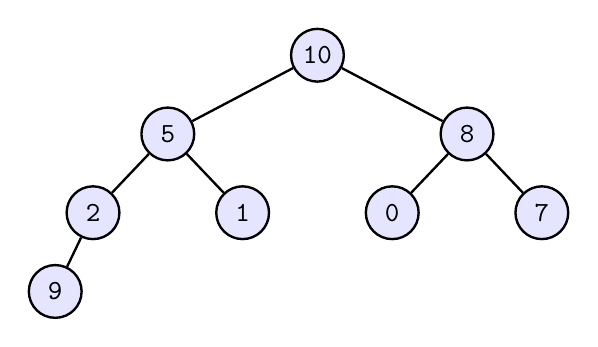
\begin{tikzpicture}

\fill[blue!10] (0.0, 0.0) circle (0.35);
\node [line width=0.03cm,black,minimum size=0.6699999999999999cm,draw,circle] at (0.0,0.0)(10){};\draw (0.0, 0.0) node[color=black] {\texttt{10}};
\fill[blue!10] (-1.9, -1.0) circle (0.35);
\node [line width=0.03cm,black,minimum size=0.6699999999999999cm,draw,circle] at (-1.9,-1.0)(5){};\draw (-1.9, -1.0) node[color=black] {\texttt{5}};
\fill[blue!10] (1.9, -1.0) circle (0.35);
\node [line width=0.03cm,black,minimum size=0.6699999999999999cm,draw,circle] at (1.9,-1.0)(8){};\draw (1.9, -1.0) node[color=black] {\texttt{8}};
\fill[blue!10] (-2.85, -2.0) circle (0.35);
\node [line width=0.03cm,black,minimum size=0.6699999999999999cm,draw,circle] at (-2.85,-2.0)(2){};\draw (-2.85, -2.0) node[color=black] {\texttt{2}};
\fill[blue!10] (-0.95, -2.0) circle (0.35);
\node [line width=0.03cm,black,minimum size=0.6699999999999999cm,draw,circle] at (-0.95,-2.0)(1){};\draw (-0.95, -2.0) node[color=black] {\texttt{1}};
\fill[blue!10] (0.95, -2.0) circle (0.35);
\node [line width=0.03cm,black,minimum size=0.6699999999999999cm,draw,circle] at (0.95,-2.0)(0){};\draw (0.95, -2.0) node[color=black] {\texttt{0}};
\fill[blue!10] (2.85, -2.0) circle (0.35);
\node [line width=0.03cm,black,minimum size=0.6699999999999999cm,draw,circle] at (2.85,-2.0)(7){};\draw (2.85, -2.0) node[color=black] {\texttt{7}};
\fill[blue!10] (-3.33, -3.0) circle (0.35);
\node [line width=0.03cm,black,minimum size=0.6699999999999999cm,draw,circle] at (-3.33,-3.0)(9){};\draw (-3.33, -3.0) node[color=black] {\texttt{9}};\draw[line width=0.03cm,black] (10) to  (5);
\draw[line width=0.03cm,black] (10) to  (8);
\draw[line width=0.03cm,black] (5) to  (2);
\draw[line width=0.03cm,black] (5) to  (1);
\draw[line width=0.03cm,black] (8) to  (0);
\draw[line width=0.03cm,black] (8) to  (7);
\draw[line width=0.03cm,black] (2) to  (9);
\end{tikzpicture}

\end{center}



It's easy to see that in the DFA, the $a$--
and $b$--transitions from the state $\{\}$ goes back to itself.
Therefore the completed DFA is this:


\begin{center}
\begin{tikzpicture}[>=triangle 60,shorten >=0.5pt,node distance=2cm,auto,initial text=, double distance=2pt]
\node[state,initial] (A) at (  0,  0) {$\{q_0\}$};
\node[state] (B) at (  3,  0) {$\{\}$};

\path[->]
(A) edge [bend left=0,pos=0.5,above] node {$a,b$} (B)
(B) edge [loop above] node {$a,b$} ()

;
\end{tikzpicture}
\end{center}
    



\newpage

Solution to Exercise \ref{ex:dfa-as-powerful-as-nfa1}\labeltext{}{sol:dfa-as-powerful-as-nfa1}.

\tinysidebar{\debug{exercises/{dfa-as-powerful-as-nfa1/answer.tex}}}

    Solution not provided.
    

\newpage

Solution to Exercise \ref{ex:dfa-as-powerful-as-nfa2}\labeltext{}{sol:dfa-as-powerful-as-nfa2}.

\tinysidebar{\debug{exercises/{dfa-as-powerful-as-nfa2/answer.tex}}}

    Solution not provided.
    

\newpage

Solution to Exercise \ref{ex:dfa-as-powerful-as-nfa3}\labeltext{}{sol:dfa-as-powerful-as-nfa3}.

\tinysidebar{\debug{exercises/{dfa-as-powerful-as-nfa3/answer.tex}}}

    Solution not provided.
    

\newpage

Solution to Exercise \ref{ex:dfa-as-powerful-as-nfa4}\labeltext{}{sol:dfa-as-powerful-as-nfa4}.

\tinysidebar{\debug{exercises/{dfa-as-powerful-as-nfa4/answer.tex}}}

    Solution not provided.
    

\newpage

Solution to Exercise \ref{ex:closure0}\labeltext{}{sol:closure0}.

\tinysidebar{\debug{exercises/{closure0/answer.tex}}}

    Solution not provided.
    

\newpage

Solution to Exercise \ref{ex:closure1}\labeltext{}{sol:closure1}.

\tinysidebar{\debug{exercises/{closure1/answer.tex}}}

    Solution not provided.
    

\newpage

Solution to Exercise \ref{ex:closure2}\labeltext{}{sol:closure2}.

\tinysidebar{\debug{exercises/{closure2/answer.tex}}}

    Solution not provided.
    

\newpage

Solution to Exercise \ref{ex:closure3}\labeltext{}{sol:closure3}.

\tinysidebar{\debug{exercises/{closure3/answer.tex}}}

    Solution not provided.
    

\newpage

Solution to Exercise \ref{ex:closure4}\labeltext{}{sol:closure4}.

\tinysidebar{\debug{exercises/{closure4/answer.tex}}}

    Solution not provided.
    

\newpage

Solution to Exercise \ref{ex:closure5}\labeltext{}{sol:closure5}.

\tinysidebar{\debug{exercises/{closure5/answer.tex}}}

    Solution not provided.
    

\newpage

Solution to Exercise \ref{ex:closure6}\labeltext{}{sol:closure6}.

\tinysidebar{\debug{exercises/{closure6/answer.tex}}}

    Solution not provided.
    

\newpage

Solution to Exercise \ref{ex:closure7}\labeltext{}{sol:closure7}.

\tinysidebar{\debug{exercises/{closure7/answer.tex}}}

    Solution not provided.
    

\newpage

Solution to Exercise \ref{ex:closure8}\labeltext{}{sol:closure8}.

\tinysidebar{\debug{exercises/{closure8/answer.tex}}}

    Solution not provided.
    

\newpage

Solution to Exercise \ref{ex:closure9}\labeltext{}{sol:closure9}.

\tinysidebar{\debug{exercises/{closure9/answer.tex}}}

    Solution not provided.
    

\newpage

Solution to Exercise \ref{ex:closure10}\labeltext{}{sol:closure10}.

\tinysidebar{\debug{exercises/{closure10/answer.tex}}}

    Solution not provided.
    

\newpage

Solution to Exercise \ref{ex:closure11}\labeltext{}{sol:closure11}.

\tinysidebar{\debug{exercises/{closure11/answer.tex}}}

    Solution not provided.
    

\newpage

Solution to Exercise \ref{ex:closure12}\labeltext{}{sol:closure12}.

\tinysidebar{\debug{exercises/{closure12/answer.tex}}}

    Solution not provided.
    

